\chapter{Super-Resolução Pós-Inversão Sísmica}
\label{cap:3modeloHibrido}

Neste Capítulo é apresentada a metodologia discutida neste trabalho.
São apresentadas as estratégias iniciais de aplicação do modelo convolucional,
os resultados preliminares e o cronograma de atividades.

\section{Modelo de Super-Resolução}

No capítulo anterior foi apresentado o método de inversão acústica que
representa o estado da arte no cálculo do máximo \textit{a posteriori} (MAP) para determinar o
resultado mais provável para impedância acústica \citep{Buland01012003, leandroGRSL}.
Foram apresentados os trabalhos relacionados com o desenvolvimento de modelos de redes neurais
convolucionais para tratar problemas de
super-resolução \citep{Oord16,He2016,DahlNS17}. Esta proposta investiga o emprego de um modelo de rede neural convolucional
para aumentar a resolução das imagens de impedância acústica
obtidas pelo processo de inversão sísmica. Com esta abordagem se espera obter um ganho
quantitativo, através da inserção de altas frequências no espectro de frequência da
propriedade acústica, e qualitativo, com a entrega de imagens com maior definição entre camadas.
Além disto, por se tratar de um problema de inversão, um estudo de incerteza sobre os
resultados das redes convolucionais será realizado sobre os resultados.

O modelo apresentado por \cite{DahlNS17} admite que cada \textit{pixel} pode assumir valores discretos entre
$0$ e $255$, e funciona como uma rede classificadora nesta faixa de valores. Nesta proposta,
se deseja modificar este modelo para que seja capaz de realizar regressão
diretamente sobre os valores de impedância, ou para impedância normalizada no intervalo real
$[-1,+1]$. Com isto, se espera abandonar a discretização da impedância utilizada
nos experimentos iniciais, uma vez que esta medida leva à perda de informação. 
Embora os autores pontuem as dificuldades para implementação de um modelo regressivo,
se acredita ser razoável realizar uma nova investigação sobre a implementação de um
modelo convolucional que realize a previsão para valores contínuos. Esta adaptação
passa pela substituição da função de \textit{softmax} e modificação da função de custo.

Para realizar a inversão acústica é necessário ter disponível a sísmica, a \textit{wavelet}
e o modelo de baixa frequência para impedância acústica ($<8Hz$). %(Equação \ref{eqn:mapSolution}).
A união de ambos os processos, inversão e treinamento da rede de super-resolução,
pode ser sintetizada de acordo com as seguintes etapas:
\begin{enumerate}
  \item Parametrização do método de inversão acústica com a sísmica, a \textit{wavelet} e o modelo de baixa frequência.
  \item Aplicação da inversão MAP para gerar as imagens de baixa resolução.
  \item Formação dos pares de imagens de treinamento: impedância invertida(sem alta frequência) e impedância sintética
  (com alta frequência).
  \item Divisão do conjunto de dados entre conjunto de treinamento e conjunto de teste.
  \item Treinamento do modelo de rede convolucional com os pares de imagens de treinamento.
  \item Aplicação da rede treinada ao conjunto de imagens usadas para teste.
  \item Comparação entre as imagens obtidas da rede e as imagens reais.
\end{enumerate}

A rede convolucional é um modelo cujo treinamento é supervisionado, de modo que,
para otimizar seus parâmetros, é necessário dispor dos pares de imagens de alta
e baixa resolução. Uma vez a rede convolucional treinada, é possível aumentar a
resolução de imagens provenientes de outros cenários da inversão acústica.

\section{Resultados Preliminares}
Os primeiros experimentos exploraram o potencial do modelo de rede convolucional que representa
o estado da arte em super-resolução. Este modelo foi adaptado para realizara super-resolução
sobre dois conjuntos de dados sintéticos. O primeiro conjunto de dados representa uma estrutura
geológica em formato de cunha envolto de uma segunda estrutura.
O segundo conjunto consiste em um cubo de impedâncias sintéticas usadas para realizar a inversão
sísmica para a própria impedância. Em ambos os casos foram separadas $25$ imagens para testes,
de modo que elas não foram utilizadas durante a fase de treinamento da RNC. Para ilustrar os resultados
no texto, as $25$ imagens de teste, de dimensões $32$ x $32$, foram agrupados em uma única imagem de $160 x 160$. 

Os valores de impedância foram discretizadas para o intervalo entre $0$ e $255$, com a aplicação da Equação \ref{eqn:norm_im}:
\begin{equation}
 K_{(i,j)} = \floor*{\big( \frac{256*(I_{i,j} - min(I))}{max(I)} \big)},
\label{eqn:norm_im}
 \end{equation}
onde $I_{i,j}$ é a intensidade do \textit{pixel} na posição $(i,j)$ da imagem $I$,
$max(I)$ é o \textit{pixel} de maior intensidade e $min(I)$ é o \textit{pixel} de menor intensidade
na imagem $I$. Os valores $min(I)$ e $max(I)$ foram armazenados, de modo que é
possível recuperar os valores de impedância das imagens de alta resolução obtidas da rede,
através da aplicação da relação inversa da Equação \ref{eqn:norm_im}. Entretanto,
a função de arredondamento utilizada leva à perda de informação.

\subsection{Caso sintético: Cunha}
No exemplo da \textit{cunha}, foram geradas $640$ imagens de tamanho $32$ x $32$ da estrutura geológica em forma
de cunha, perfazendo um total de $20$ grupos de treinamento. Adicionalmente, foram geradas $32$
novas imagens para teste da rede. As estruturas criadas correspondem a valores de impedância
acústica em função da profundidade e representam um conjunto de dados simples, pois as camadas são uniformes,
de modo que todo os pontos de uma camada possuem o mesmo valor de impedância.

Para gerar o conjunto de imagens de baixa resolução, as imagens de alta resolução foram filtradas por meio de filtro
passa baixa, com frequência de corte em $4Hz$. A Figura \ref{fig:cunhas} apresenta um conjunto exemplo
usado no treinamento da rede convolucional para o caso em questão. A Figura \ref{fig:cunhahr} exibe
a cunha sintética em alta resolução e a Figura \ref{fig:cunhalr} apresenta a mesma cunha filtrada.
\begin{figure}[ht]
\centering
\begin{subfigure}{.8\textwidth}
  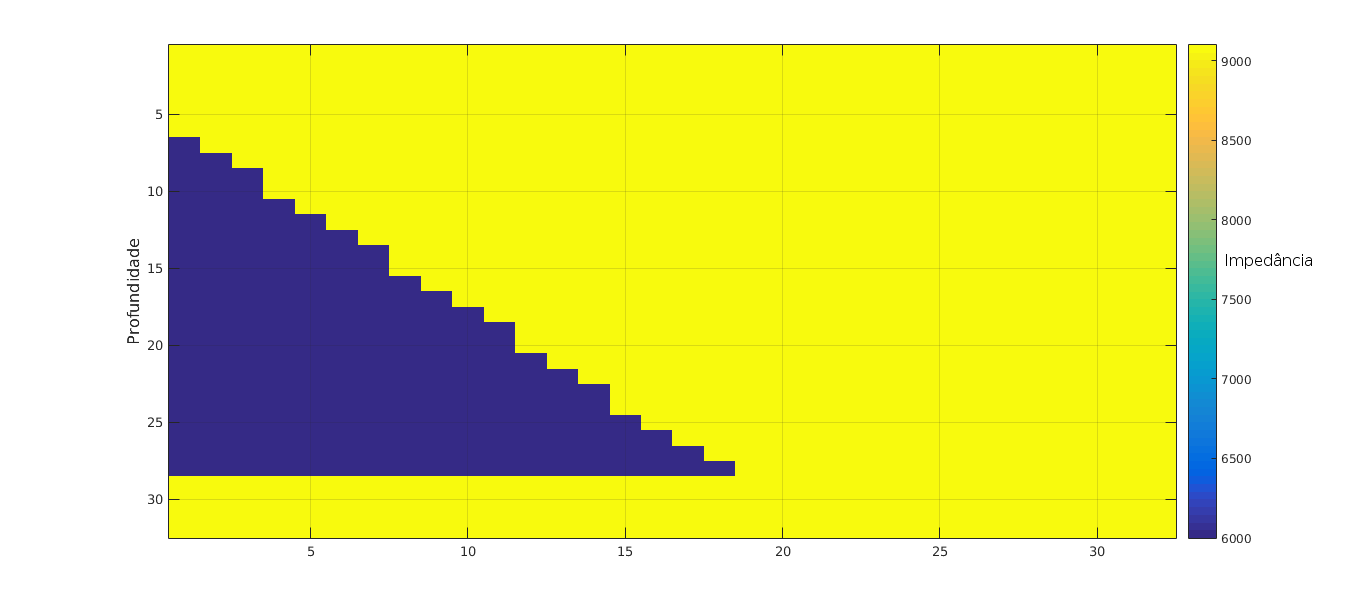
\includegraphics[width=.9\linewidth]{fig/cunha_hr}
  \caption{Cunha em alta resolução.}
  \label{fig:cunhahr}
\end{subfigure}
\begin{subfigure}{.8\textwidth}
  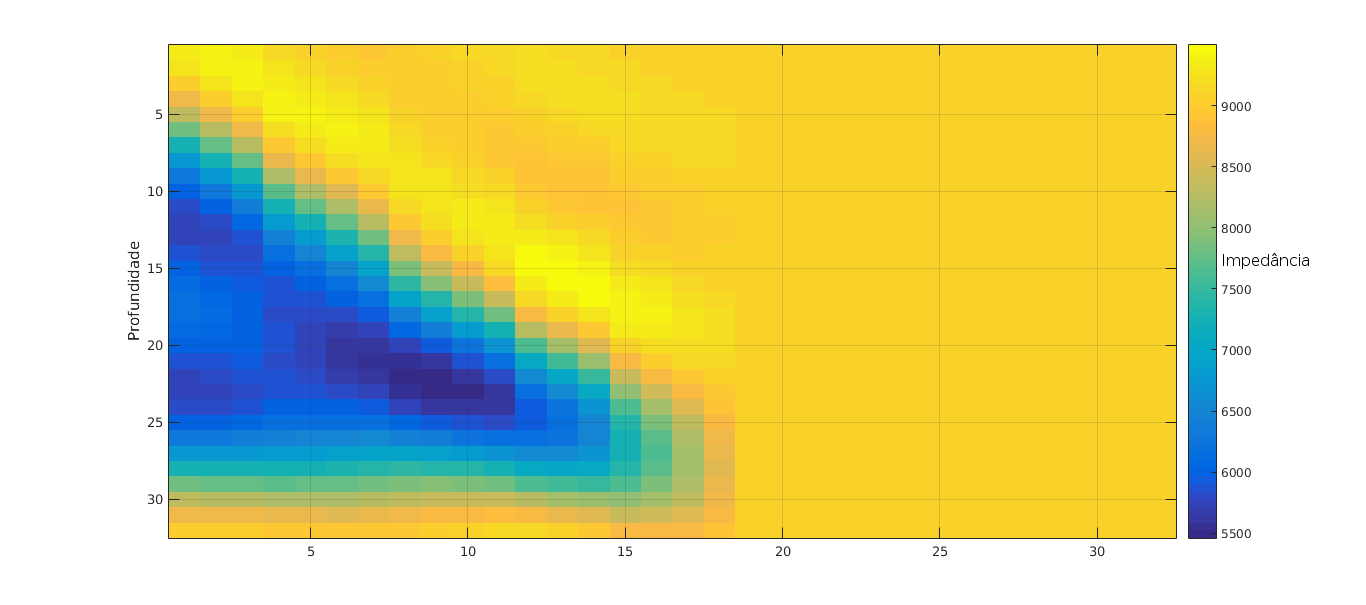
\includegraphics[width=.9\linewidth]{fig/cunha_lr}
  \caption{Cunha em baixa resolução.}
  \label{fig:cunhalr}
\end{subfigure}%
\caption{Exemplo de um conjunto de treinamento da rede convolucional.}
\label{fig:cunhas}
\end{figure}

Nas Figuras \ref{fig:result_cunha_pixel}, \ref{fig:cunha_pixel_hr} e \ref{fig:cunha_pixel_lr} é possível comparar
o resultado da super-resolução com a imagem sintética da cunha. Na Figura \ref{fig:result_cunha_pixel} são
apresentadas as imagens obtidas na saída da rede convolucional, na Figura \ref{fig:cunha_pixel_hr} são
apresentadas as imagens de referência em alta resolução e na Figura \ref{fig:cunha_pixel_lr} são apresentas
as imagens filtradas em baixa resolução. Estas imagens fazem parte do conjunto de teste,
de modo que não foram utilizadas durante o treinamento da rede. 

\begin{figure}[ht]
\centering
\begin{subfigure}{.8\textwidth}
 \centering
  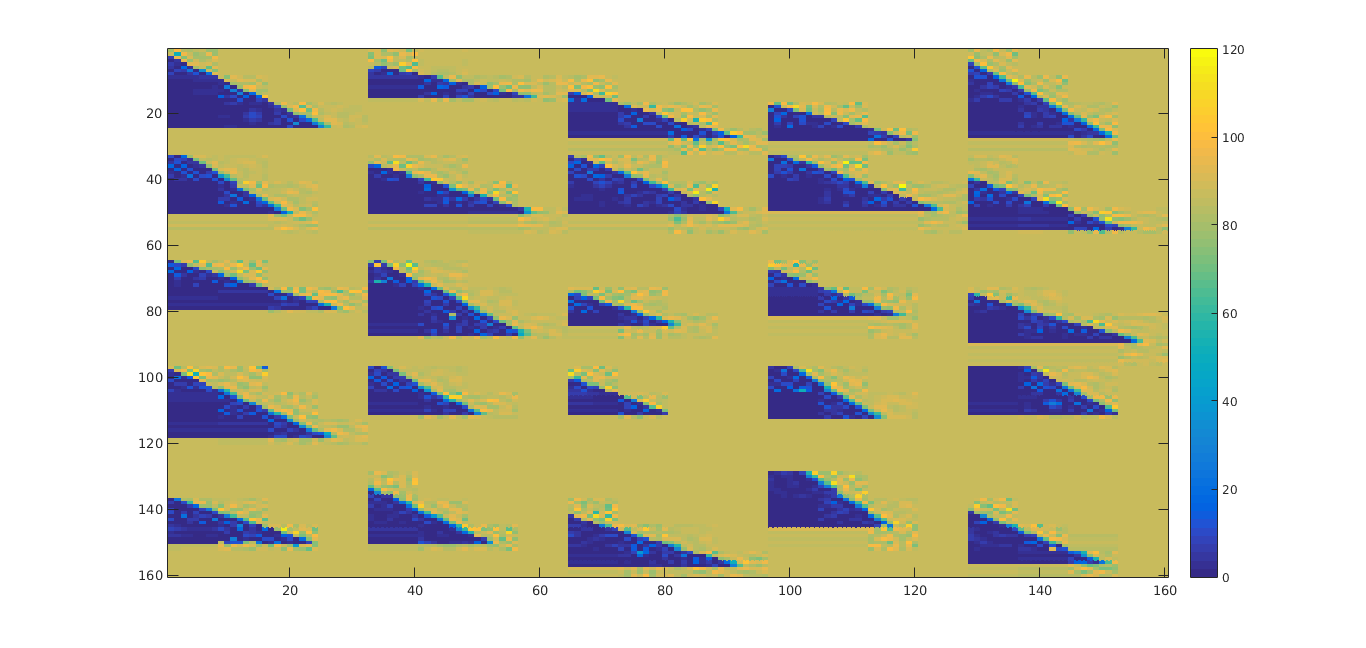
\includegraphics[width=.7\linewidth]{fig/result_cunha_pixel}
  \caption{Imagens de cunhas em super-resolução.}
  \label{fig:result_cunha_pixel}
\end{subfigure}

\begin{subfigure}{.8\textwidth}
 \centering
  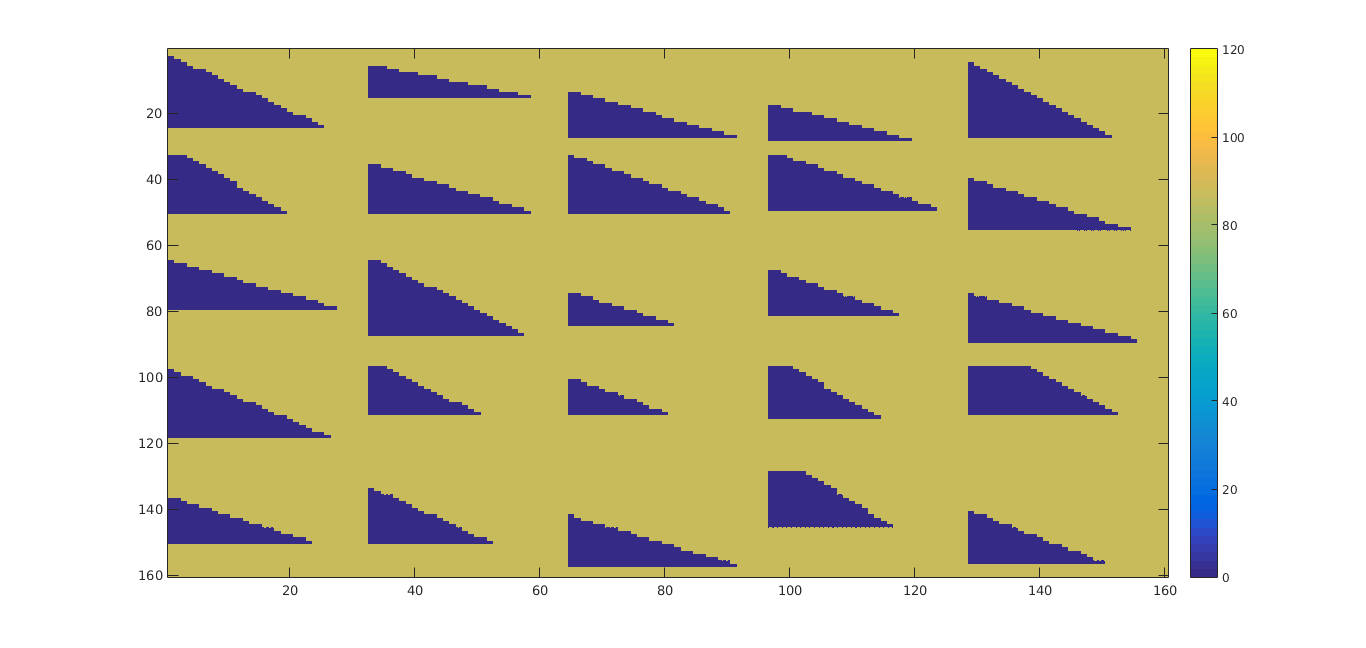
\includegraphics[width=.7\linewidth]{fig/cunha_pixel_hr}
  \caption{Imagens de cunhas em alta resolução.}
  \label{fig:cunha_pixel_hr}
\end{subfigure}

\begin{subfigure}{.8\textwidth}
  \centering
  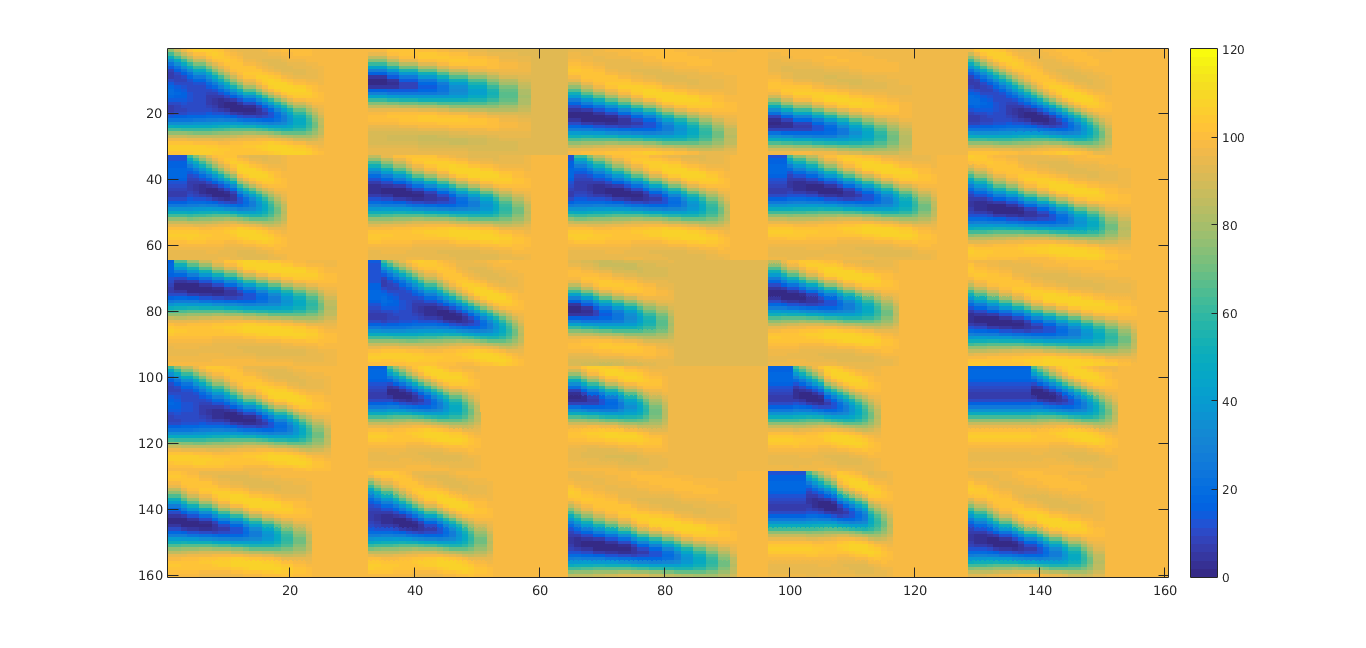
\includegraphics[width=.7\linewidth]{fig/cunha_pixel_lr}
  \caption{Imagens de cunhas em baixa resolução.}
  \label{fig:cunha_pixel_lr}
\end{subfigure}
\end{figure}

Para este exemplo inicial apenas a avaliação qualitativa foi realizada e se observa que a rede foi capaz de 
identificar e aprender as estruturas observadas das imagens de baixa resolução. A resolução foi
aumentada, mas se observa algumas regiões de incerteza da rede.

\subsection{Caso sintético: Impedância Acústica}
Para realizar o segundo experimento foi utilizado um cubo sintético de impedância
acústica com $239$ imagens de dimensões $250$ x $199$. Do cubo de impedância foram calculados os
valores de refletividade. Uma \textit{wavelet}
sintética foi estimada e o cubo sísmico foi obtido por meio da
convolução entre a refletividade e a \textit{wavelet}. O cubo de impedância 
foi filtrado abaixo de $8Hz$ para obter o modelo de baixa frequência e
um ruído foi adicionado à sísmica. O método de inversão acústica por MAP
foi parametrizado para disponibilizar imagens com nível elevado de ruído.
Esta medida visou resultados que pudessem ser avaliados sob a perspectiva qualitativa e quantitativa.
Na figura \ref{fig:ipedances} estão ilustrados os exemplos de pares de imagens de alta e baixa resolução.
Por conta das limitações de memória de processamento, foi necessário realizar um recorte das imagens de impedância
obtidas da inversão. Para efeito de teste do modelo, foram utilizadas imagens com dimensões $32$ x $32$ do cubo de impedância.
O recorte realizado nas imagens compreendeu as regiões de provável reservatório, como ilustrado nas Figuras \ref{fig:impedancehr}
e \ref{fig:impedancelr}.

\begin{figure}[ht]
\centering
\begin{subfigure}{.8\textwidth}
  \centering
  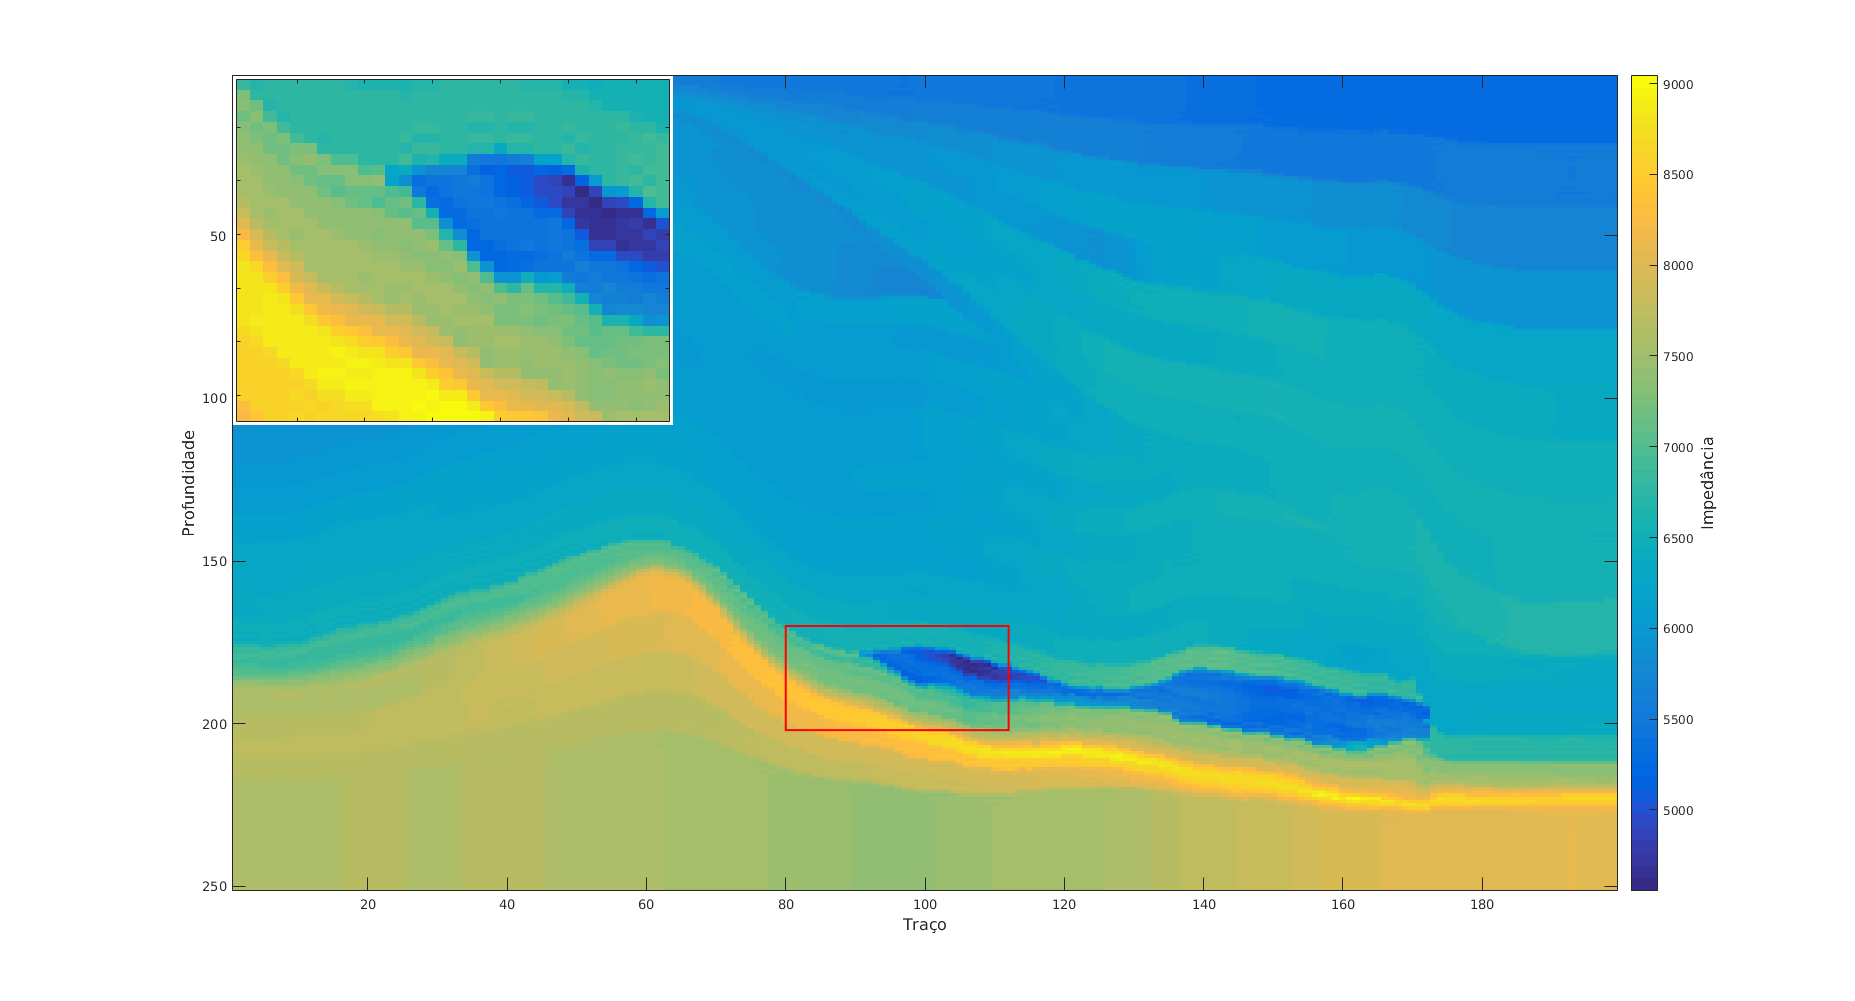
\includegraphics[width=.9\linewidth]{fig/impedance_mount}
  \caption{Seção do cubo de impedância sintética.}
  \label{fig:impedancehr}
\end{subfigure}
\begin{subfigure}{.8\textwidth}
  \centering
  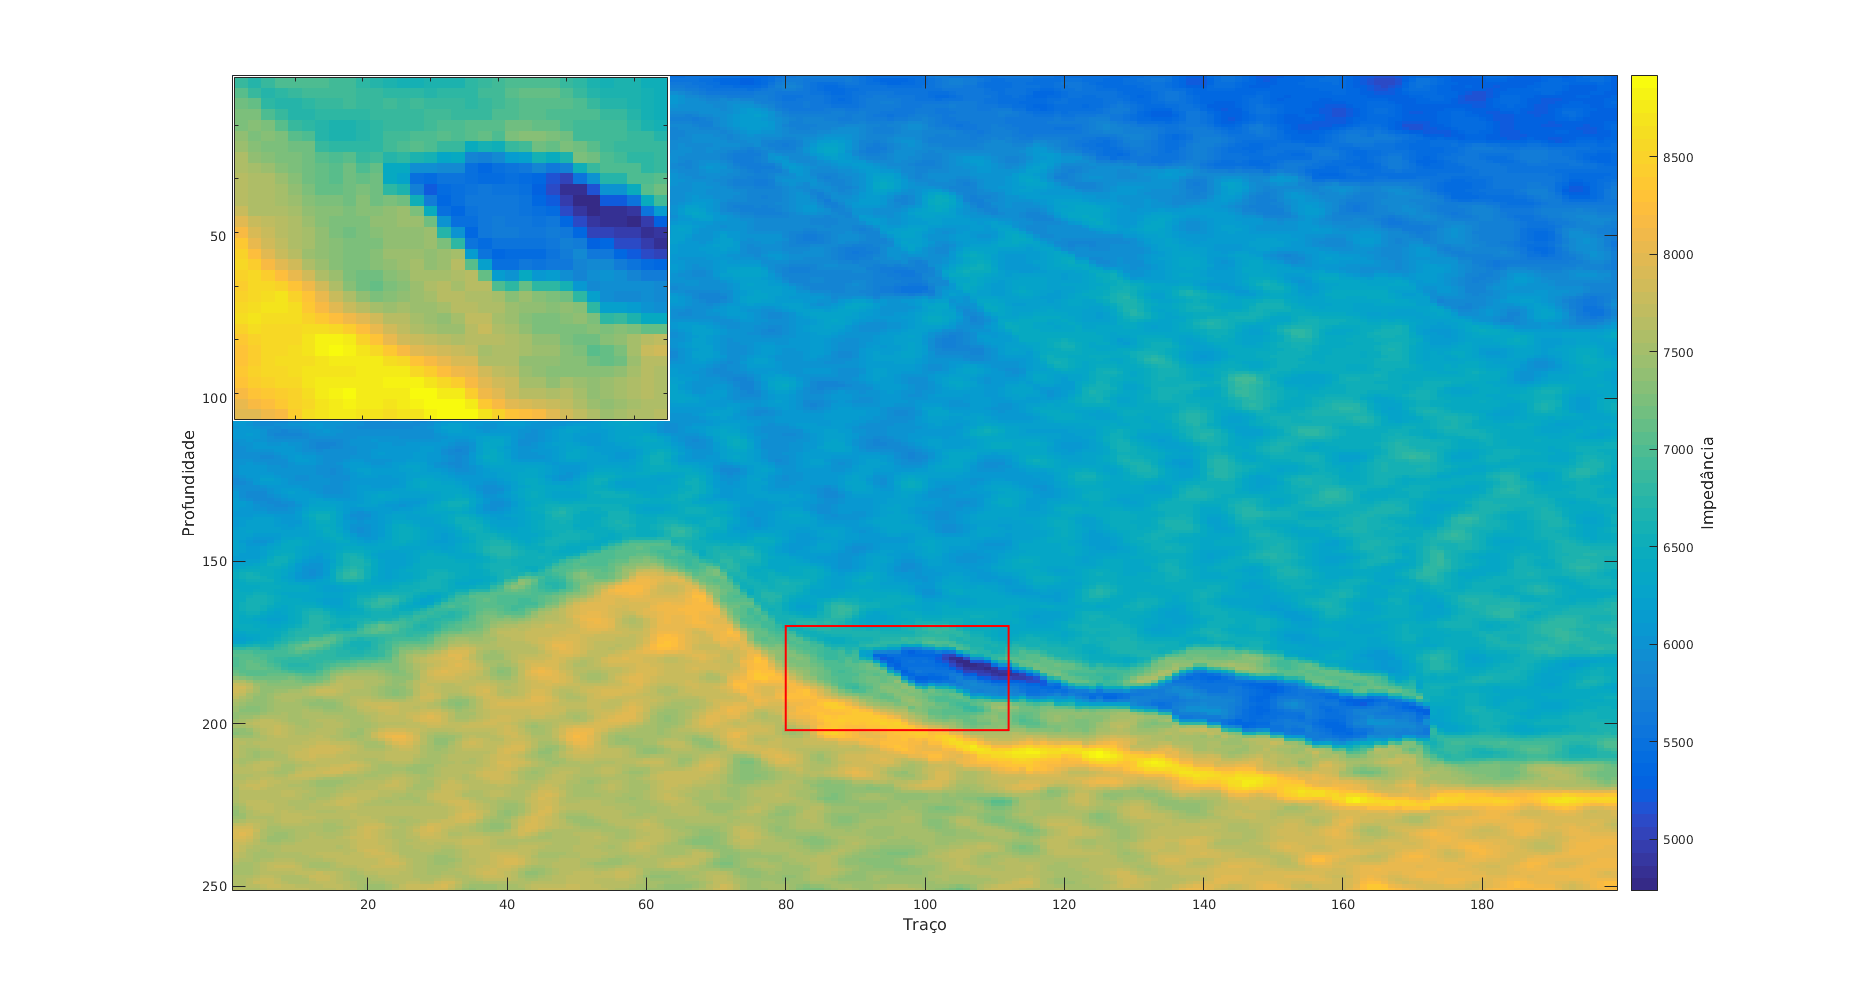
\includegraphics[width=.9\linewidth]{fig/inversion_mount}
  \caption{Resultado da inversão para a mesma seção do cubo.}
  \label{fig:impedancelr}
\end{subfigure}%
\caption{Seção do cubo de impedância da inversão MAP.}
\label{fig:ipedances}
\end{figure}

As redes convolucionais foram treinadas por 16 mil iterações e o modelo se mostrou convergente,
a Figura
\ref{fig:inversionhr} apresenta o resultado da RNC, a Figura \ref{fig:inversionhr} os recortes da impedância sintética e a
Figura \ref{fig:inversionlr} apresenta os recortes das imagens obtidas pelo processo de inversão
por MAP. A quantidade elevada de erros observados na predição da rede pode estar relacionada
ao número limitado de imagens de treinamento. Além disto, o erro da predição no conjunto de teste
é, frequentemente, maior que o erro da predição dentro do conjunto de treinamento. Se o número de imagens
de treinamento é pequeno, a rede pode ser levada a prever estruturas desconhecidas no conjunto
de teste e sua capacidade preditiva se tornar limitada. Por outro lado, nas regiões reconhecidas pela rede
o ruido, que era visível na inversão, foi filtrado e as camadas se tornaram mais evidentes.
A avaliação quantitativa foi realizada utilizando uma métrica baseada no Transformada Rápida de Fourier (FFT),
discutido na seção seguinte.
\begin{figure}[ht]
\centering
\begin{subfigure}{.8\textwidth}
  \centering
  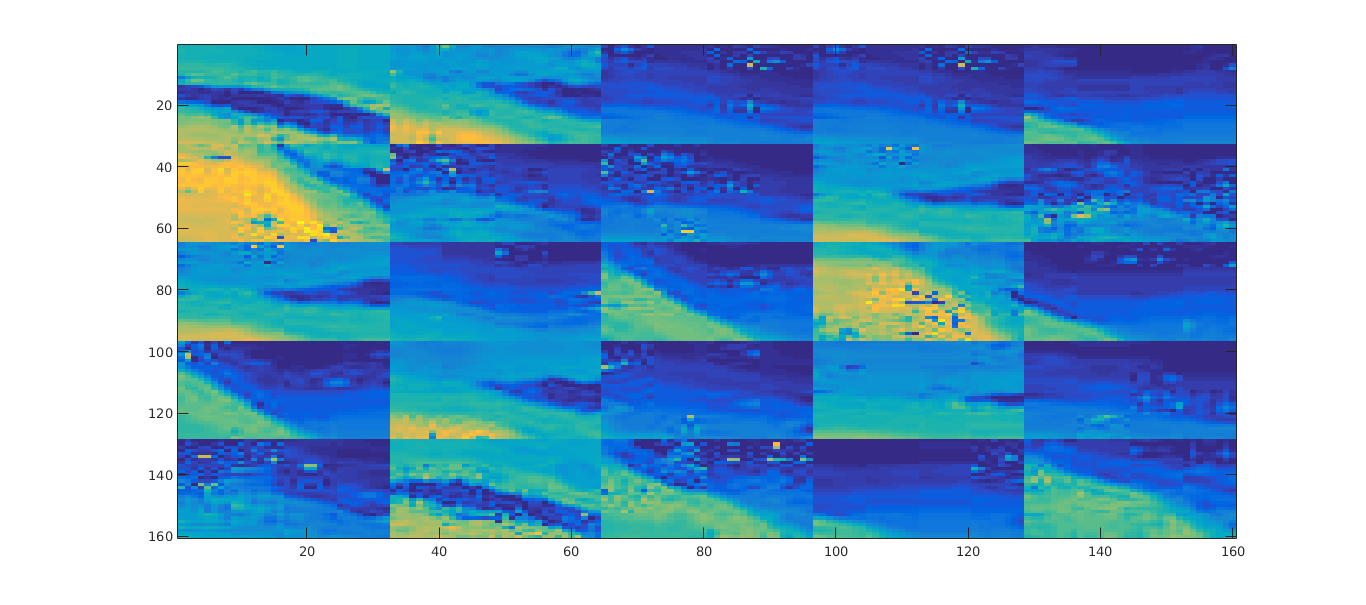
\includegraphics[width=.7\linewidth]{fig/inversion_cnn}
  \caption{Imagens obtidas por super-resolução.}
  \label{fig:inversionhr}
\end{subfigure}

\begin{subfigure}{.8\textwidth}
  \centering
  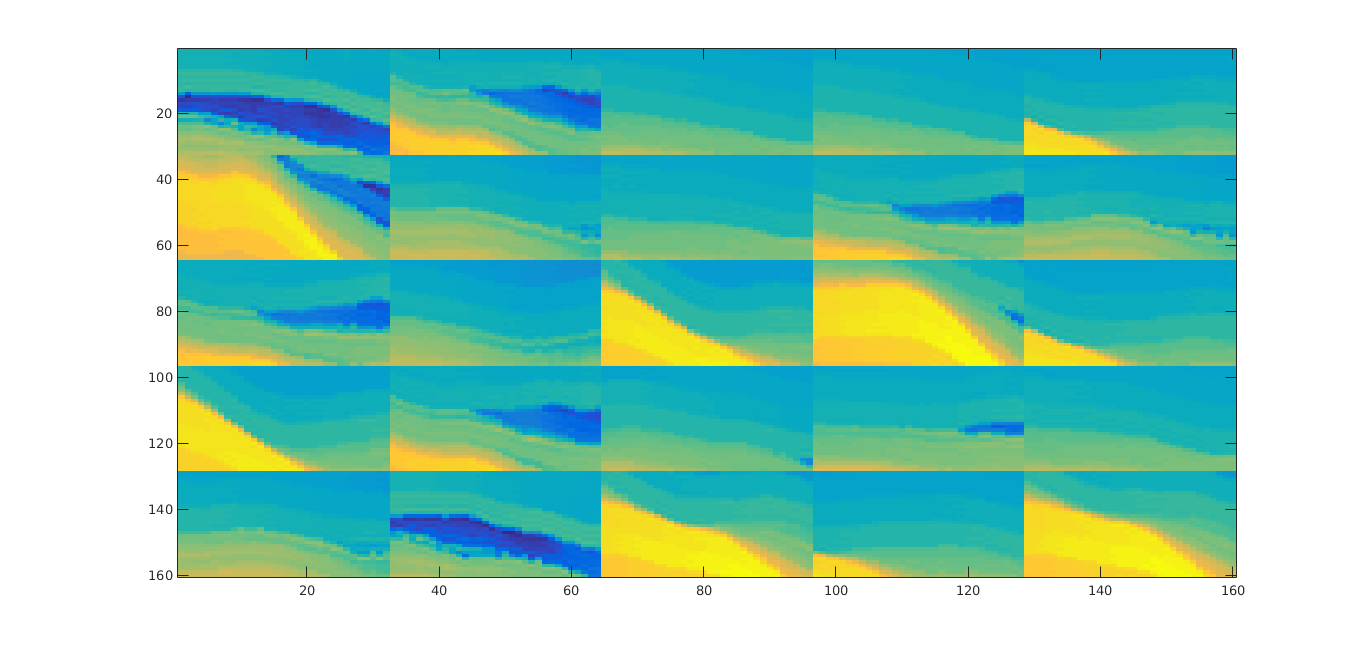
\includegraphics[width=.7\linewidth]{fig/inversion_hr_test}
  \caption{Imagens da impedância sintética.}
  \label{fig:hr}
\end{subfigure}
\begin{subfigure}{.8\textwidth}
  \centering
  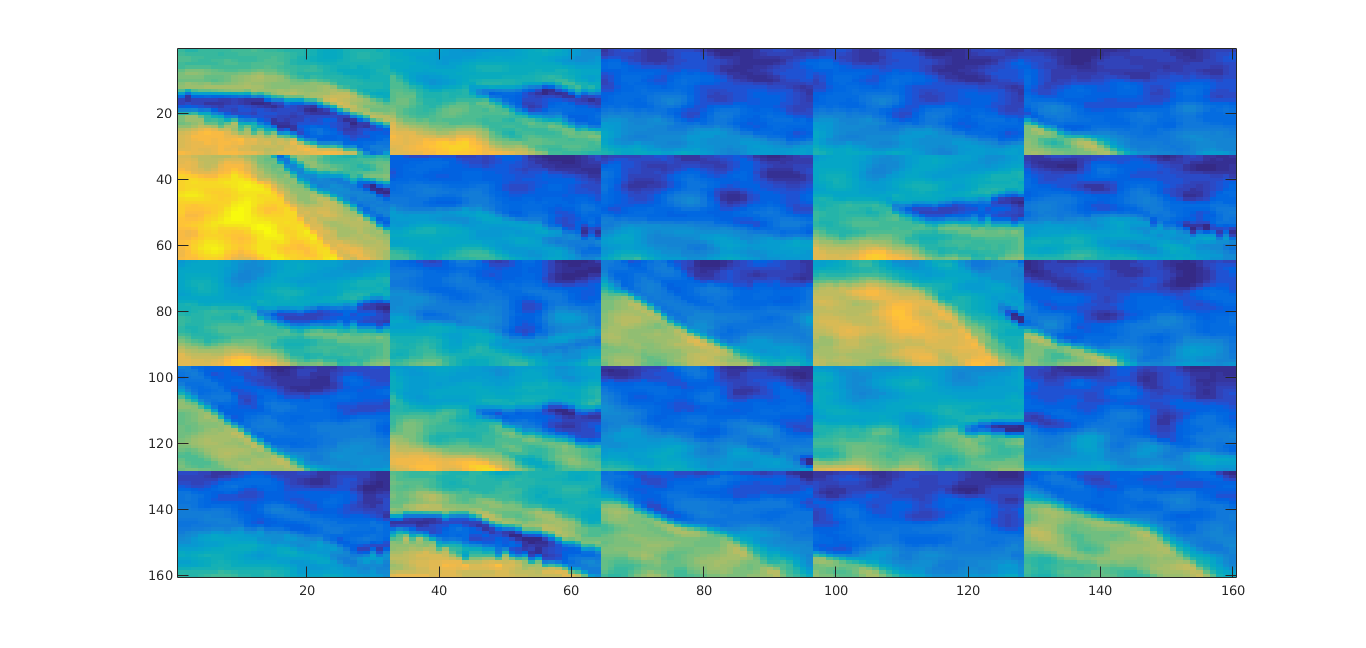
\includegraphics[width=.7\linewidth]{fig/inversion_map}
  \caption{Imagens da inversão por MAP.}
  \label{fig:inversionlr}
\end{subfigure}%
\label{fig:inversions}
\end{figure}

Uma estratégia para lidar com a limitação de memória de processamento é definir uma janela deslizante sobre as imagens, de
modo que cada imagem seja dividida em um novo conjuntos de treinamento composto por sub-imagens e a mesma rede pode
aprender com base nas sub-imagens. Um conjunto de sub-imagens pode ser usada para teste e, ao final, a imagem em tamanho
original é reconstruída a partir das sub-imagens de alta resolução obtidas pela rede.

\subsection{Transformada Rápida de Fourier}

A Transformada Rápida de Fourier (FFT) foi utilizada para avaliação quantitativa e comparação entre as imagens calculadas pela rede
e as imagens de alta resolução de impedância sintética. A métrica de similaridade entre as imagens é calculada usando
a Equação \ref{eq:fourier}, com base no espectro de frequência das imagens \citep{Narayana15}.
\begin{equation}
 C = \frac{ (\sum_{i=1}^{N}{F_{1i}F_{2i}} - N \bar{F}_1\bar{F}_2 )^2 }{ (\sum_{i=1}^{N}{|F_{1i}|^2} - N{\bar{F}^2}_1)( \sum_{i=1}^{N}{|F_{2i}|^2} - N{\bar{F}^2}_2 )},
 \label{eq:fourier}
\end{equation}

onde, para cada frequência, um valor de intensidade é obtido das partes real e complexa da Transformada de Fourier.
$F_{1i}$ é o valor de intensidade do $i$-ésimo \textit{pixel} da primeira imagem, enquanto $F_{2i}$
é o valor de intensidade do $i$-ésimo \textit{pixel} da segunda imagem. $\bar{F}_1$ e $\bar{F}_2$ representam os valores
de frequência média de cada imagem. De acordo com \cite{Narayana15}, quanto mais próximo de $1$, mais similares as imagens
comparadas.

A métrica $C$ foi calculada entre as imagens obtidas pela rede e as imagens de alta resolução de impedância sintética, também, entre estas e
as imagens de MAP de impedância (baixa resolução). Com a utilização da métrica $C$, foi possível realizar uma busca dentro do conjunto de 
imagens sintéticas, para identificar aquela que forma o par com a imagem obtida da rede. Em todos os casos a imagem encontrada era a imagem
que realmente equivale à imagem simulada. Na maioria dos casos, em torno de $84\%$, as imagens obtidas pela rede
apresentaram maior similaridade com as imagens sintéticas. Por outro lado, em cerca de $16\%$ dos casos as imagens da rede apresentaram mais similaridade com
a imagem de baixa resolução. Este fato é um indicativo de que em alguns casos a rede não foi capaz de realizar super-resolução das imagens borradas e
as causas deste evento ainda precisam ser investigadas.

Com base nos testes realizados, se notou que a métrica assume valor $1$ quando se compara duas imagens exatamente iguais.
Esta observação se deu ao comparar uma imagem com sua cópia. Entretanto, $C$ pode assumir valores negativos menores que $-1$ e estas ocorrências
não são claramente explicadas por \cite{Narayana15}, de modo que esta métrica ainda necessita ser melhor compreendida. É necessário
um estudo de dissimilaridade entre imagens para a compreensão mais ampla da faixa de valores admissíveis por $C$ e seus significados.

\section{Proposta e Plano de Trabalho}

Os resultados preliminares indicam ser possível obter imagens de
inversão acústica em maior resolução. Entretanto, a aplicabilidade
do modelo depende da existência do conjunto de pares de imagens
de alta e baixa resolução suficientemente grande para o treinamento da rede. Consequentemente,
o limite da capacidade de inserção de altas frequências das imagens previstas
será limitada pelo faixa de altas frequências das imagens de treinamento.

Ao final da pesquisa se espera alcançar as respostas para as seguintes questões:
\begin{itemize}
 \item O modelo de rede convolucional é capaz de aumentar a resolução de imagens de impedância acústica
quantitativamente?
 \item As imagens de teste apresentaram maior resolução que as imagens originais, sob o ponto 
de vista de altas frequências?
 \item Como as redes neurais aprendem as altas frequências?
 \item É possível parametrizar o processo de super-resolução para imagens pós-inversão?
 \item Quais faixas de alta frequências são inseridas?
 \item Qual limite de alta frequência é possível inserir nas imagens de alta resolução?
 \item Existe coerência geoestatística no resultado do modelo convolucional?
 \item O modelo é expansível para outros tipos de propriedades petrofísicas?
\end{itemize}

A proposta para o restante do projeto é obter resultados mais consistentes com o modelo de teste atual,
implementar a rede convolucional para realizar super-resolução sobre valores contínuos, definir uma estratégia para
a análise de incerteza sobre os resultados da rede convolucional, adaptar o modelo para realizar a super-resolução
de imagens em dimensões maiores que $32$ x $32$ e analisar o comportamento da rede para inversão
com um conjunto de dados reais.

O caráter de originalidade do trabalho é garantido pelas contribuições para as
áreas de aprendizagem por redes neurais convolucionais e inversão sísmica.
A primeira contribuição está relacionada com o desenvolvimento de um
novo modelo de rede convolucional para super-resolução.
A segunda contribuição será a disponibilização de um método capaz de
proporcionar imagens da inversão acústica em maior resolução que auxiliem
na tomada de decisão na caracterização de reservatório. Além disso, a modelagem
das incertezas nos dados de saída da RNC permitirá um entendimento sobre que tipo de modificações
ocorreram e quais frequências inseridas pela RNC passaram a existir
nas imagens de alta resolução, mas que não estavam presentes nas imagens de baixa resolução.
O caráter de ineditismo é garantido, pois não se verificou na literatura uma
abordagem de super-resolução para a inversão sísmica que permita um
ganho quantitativo e qualitativo das imagens da propriedade invertida.
O caráter de não-trivialidade é observado, pois a implementação do modelo
envolve aspectos técnicos complexos como formalismos matemáticos, estudo
de incerteza e generalização do modelo.

Dentre os periódicos que apresentam trabalhos relacionados com esta área, se
destacam os seguintes com suas classificações no Qualis para Ciências da
Computação:

\begin{itemize}
  \setlength{\itemsep}{0pt}
  \setlength{\parskip}{0pt}
  \item IEEE Trans. on Geoscience and Remote Sensing
  \item ISSN: 0196-2892 - IEEE - Qualis A1
\end{itemize}

\begin{itemize}
  \setlength{\itemsep}{0pt}
  \setlength{\parskip}{0pt}
  \item Journal of Computational Physics
  \item ISSN: 0021-9991 - Elsevier - Qualis A1
\end{itemize}

\begin{itemize}
  \setlength{\itemsep}{0pt}
  \setlength{\parskip}{0pt}
  \item Pattern Recognition
  \item ISSN: 0031-3203 - Elsevier - Qualis A1
\end{itemize}


\begin{itemize}
  \setlength{\itemsep}{0pt}
  \setlength{\parskip}{0pt}
  \item Pattern Recognition Letters
  \item ISSN: 0167-8655 - Springer - Qualis A1
\end{itemize}

% 
% \begin{itemize}
%   \setlength{\itemsep}{0pt}
%   \setlength{\parskip}{0pt}
%   \item Geophysics
%   \item ISSN: 0016-8033 - Society of Exploration Geophysicists - Qualis A2 Interdisciplinar
% \end{itemize}
% 
% 
% \begin{itemize}
%   \setlength{\itemsep}{0pt}
%   \setlength{\parskip}{0pt}
%   \item Mathematical Geosciences
%   \item ISSN: 1874-8961 - Springer - Qualis A2 Interdisciplinar
% \end{itemize}

